\documentclass{article}

\usepackage[a4paper, margin=2cm]{geometry}
\usepackage[utf8]{inputenc}

\usepackage[czech]{babel}
\usepackage{fvextra}
\usepackage{csquotes}
\usepackage{parskip}
\usepackage{expl3}

\usepackage{float}
\usepackage{amsmath}
\usepackage{enumitem}

\usepackage{minted}

\usepackage{graphicx}
\graphicspath{{images}}

\usepackage[hidelinks, unicode, pdfusetitle]{hyperref}

\title{Atlas a rejstřík zlomků}
\author{Benjamin Swart}

\begin{document}

\maketitle

\section{Zadání}

Máme za úkol vygenerovat Fareyovu posloupnost, a to nejprve celou, a poté prvních $k$ prvků.

Parametry $N$ a $K$ jsem přejmenoval na $n$ a $k$, jelikož budu velkými písmeny značit množiny a posloupnosti.

\section{Generace celé posloupnosti (35-1-4)}

Generace celé Fareyovy posloupnosti je snazší, než generace její části, protože můžeme prvky vygenerovat v libovolném pořadí. Celkový počet vygenerovaných zlomků označíme $k$, podobně jako v druhé úloze.

\subsection{Pomocné výpočty}
\label{section:sieve}

Nejprve použijeme Eratosthenovo síto k tomu, abychom našli prvočíselný rozklad\footnote{Nejedná se o prvočíselný rozklad v pravém slova smyslu, ale jen o seznam prvočíselných dělitelů bez jejich mocnin. Nám to však stačí.} všech přirozených čísel od $2$ do $n$. Tradiční verze síta sice jen vrací seznam prvočísel, ale mi algoritmus upravíme, aby místo škrtání čísel ke každému postupně připisoval jeho prvočíselné dělitele.

Postup je jednoduchý. Procházíme čísla od $2$ do $n$. Pro každé číslo $a$ nejprve zkontrolujeme, jestli je prvočíslo, tj. jestli jsme vedle něj ještě nenapsali žádné dělitele. Pokud ano, tak procházíme násobky $a$ menší než $n$ (včetně $a$) a ke každému připíšeme $a$. Také $a$ přidáme do seznamu prvočísel.

Prvočíselné rozklady budeme ukládat do hašovací tabulky. Seznam prvočísel bude automaticky seřazený, jelikož prvočísla objevujeme od nejmenších k největším. V nejhorším případě, kdy budou všechna čísla prvočísla,\footnote{Pokud by všechna čísla byla prvočísla, tak by tato úloha byla výrazně jednodušší.} provedeme $\sum_{a=2}^{n}{\frac{n}{a}}$ kroků, takže složitost algoritmu bude nejhůře $O\left(n \log{n}\right)$.\footnote{Je dokázáno, že skutečná složitost Eratosthenova síta je $O\left(n \log{\log{n}}\right)$. Pro určení časové složitosti mého algoritmu však tato horní hranice zatím postačí.}

\begin{table}[ht]
    \centering
    \begin{tabular}{|l|l|}
        \hline
        Číslo      & Rozklad    \\
        \hline
        \textbf{2} & \textbf{2} \\
        \textbf{3} & \textbf{3} \\
        4          & 2          \\
        \textbf{5} & \textbf{5} \\
        6          & 2, 3       \\
        \textbf{7} & \textbf{7} \\
        8          & 2          \\
        9          & 3          \\
        10         & 2, 5       \\
        \hline
    \end{tabular}

    \caption[Prvočíselný rozklad čísel od 2 do 10]{Prvočíselný rozklad čísel od 2 do 10. Prvočísla jsou vyznačena tučně.}
    \label{table:sieve}
\end{table}

\subsection{Dělba práce}

Zlomky můžeme vypsat v libovolném pořadí. Rozdělíme si je tedy podle jmenovatele. Nejprve vypíšeme zlomky $\frac{0}{1}$ a $\frac{1}{1}$, a poté projdeme všechny možné jmenovatele od $2$ do $n$ a najdeme pro ně všechny platné zlomky.

\subsection{Generace nesoudělných čísel}

Chceme pro nějakého jmenovatele $m$ najít všechny zlomky ve tvaru $\frac{a}{m}; a \in \left\{1, 2, 3, \dots, m\right\}$, které jsou v základním tvaru. Potřebujeme tedy najít všechna přirozená čísla pod $m$, která jsou s $m$ nesoudělná.

\subsubsection{Nalezení platných prvočísel}
\label{section:valid-primes}

Díky pomocným výpočtům ze sekce \ref{section:sieve} máme k dispozici hašovací tabulku prvočíselných dělitelů $m$, kterou pojmenujeme $P_d$, a seznam všech prvočísel menších než $m$, který pojmenujeme $P_a$.\footnote{Seznam $P_a$ začíná na začátku seznamu všech prvočísel. Jeho konec snadno najdeme v lineárním čase.} Určíme doplněk $P = P_a - P_d$, neboli seznam všech prvočísel, která se mohou vyskytovat v prvočíselném rozkladu čitatele zlomku s jmenovatelem $m$.

Vypočítat ho zvládneme v lineárním čase. Budeme procházet $P_a$ a přeskakovat prvky které se vyskytují $P_d$. Výsledný seznam bude seřazený, stejně jako $P_a$.

Doba běhu tohoto podalgoritmu se v době běhu celého algoritmu ztratí. To dokážeme snadno. Provedeme počet kroků úměrný k velikosti $P_a$. Prvky $P_a$ můžeme rozdělit na prvky $P_d$ a na prvky $P$. Prvky $P_d$ jsme vygenerovali Eratosthenovým sítem a každý z nich v celém algoritmu použijeme právě jednou. To znamená, že doba potřebná k jejich použití se ztratí v době potřebné k jejich generaci. Prvky $P$ jsou všechny sami o sobě platné čitatele zlomků, a tedy jich za běhu algoritmu bude nutně nejvýše tolik, kolik vypíšeme zlomků. Doba potřebná k jejich nalezení se tedy určitě ztratí v době potřebné k vypsání zlomků.

\subsubsection{Nalézání čísel s platným prvočíselným rozkladem}

Nyní musíme vygenerovat všechna přirozená čísla menší než $m$, která mají v prvočíselném rozkladu pouze čísla v $P$. Toho dosáhneme dynamickým programováním.

Prvky $P$ označíme $p_1$ až $p_r$. Jelikož jsme je vygenerovali seřazené, tak pro platí, že $p_a < p_{a+1}; 1 \leq a < r$.

Začneme se seřazeným seznamem všech čísel, jejichž rozklad neobsahuje žádná čísla, neboli $\left<1\right>$. Tento seznam poté doplníme čísly, jejichž rozklad obsahuje jen $p_1$, poté čísly, jejichž rozklad obsahuje jen $p_1$ nebo $p_2$, a tak dále.

\subsubsection{Rozšiřování seznamu}

Máme seřazený seznam $Q_a$ všech čísel menších než $m$, jejichž rozklad obsahuje jen prvočísla $\left\{p_1, p_2, \dots, p_{a-1}\right\}$, a máme za úkol vytvořit seřazený seznam $Q_{a+1}$, jehož čísla smí mít v rozkladu navíc i $p_a$.

Předpokládejme nejprve, že všechna tato čísla budou mít v rozkladu $p_a$ nejvýše jednou. V tom případě nám stačí procházet $Q_a$ a každé číslo $q$ násobit $p_a$. Do $Q_{a+1}$ pak přidáme jak $q$ tak $p_a q$. Jakmile $p_a q$ přesáhne $m$, tak přestaneme násobit a zbytek seznamu budeme přímo kopírovat do $Q_{a+1}$.

Tento algoritmus má několik problémů. Zaprvé může ve skutečnosti rozklad čísla obsahovat $p_a$ vícekrát, zadruhé nebude seznam $Q_{a+1}$ seřazený, jak jsme chtěli, a zatřetí poběží tento algoritmus v kvadratickém čase. Podíváme se nejprve na první z těchto problémů.

Jednoduchým řešením by bylo každé $q$ násobit $p_a$ opakovaně, a to dokud výsledek nepřesáhne $m$. Existuje však i zajímavější řešení, které vyřeší i pár dalších problémů.

Místo toho, abychom $p_a q$ násobili $p_a$ znovu hned, tak ho vrátíme zpátky do $Q_a$ (samozřejmě jen pokud $p_a q < m$), kde se k němu znovu dostaneme později. $Q_a$ tedy ve skutečnosti nebude seznam, ale prioritní fronta. $p_a q$ také nemusíme přidávat do $Q_{a+1}$, jelikož ho tam přidáme, až na něj narazíme znovu ve frontě $Q_a$.

Tím se nám vyřeší i druhý problém. Jelikož do $Q_{a+1}$ přidáváme jen nezměněné prvky z prioritní fronty, tak bude nutně seřazená.

Musíme ještě zvolit implementaci prioritní fronty. $Q_a$ získává prvky ze dvou zdrojů, a to z výstupu předchozí iterace dynamického algoritmu a z násobků prvků odebraných ze sebe sama. Zajímavé je, že oba tyto zdroje nezávisle generují čísla seřazená. Použijeme tedy ve skutečnosti dvě normální fronty $Q_a$ a $Z_a$. $Q_a$ bude obsahovat výstup předchozí iterace a $Z_a$ bude obsahovat vynásobená $q$. Jako $q$ tedy vybereme vždy menší z předků obou front.

Náš algoritmus zatím vypadá takto:

\begin{enumerate}
    \item Nechť $Q_1$ je fronta obsahující číslo $1$
    \item Pro $a$ od $1$ do $r$:
          \begin{enumerate}[label*=\arabic*.]
              \item Nechť $Z_a$ je prázdná fronta
              \item Nechť $Q_{a+1}$ je prázdná fronta
              \item Dokud $Q_a$ a $Z_a$ nejsou prázdné:
                    \begin{enumerate}[label*=\arabic*.]
                        \item Odeber nejmenší z čísel na začátku $Q_a$ nebo $Z_a$ jako $q$
                        \item Přidej $q$ na konec $Q_{a+1}$
                        \item Pokud $q p_a < m$:
                              \begin{enumerate}[label*=\arabic*.]
                                  \item Přidej $q p_a$ na konec $Z_{a}$
                              \end{enumerate}
                    \end{enumerate}
          \end{enumerate}
    \item Vrať $Q_r$
\end{enumerate}

\subsubsection{Zlepšování efektivity}

Náš algoritmus na generaci nesoudělných čísel zatím běží v kvadratickém čase, jelikož dokola kopíruje ten stejný seznam. Tomu však můžeme zamezit. Uděláme dvě změny:

\begin{enumerate}
    \item Nesoudělná čísla budeme vypisovat, jakmile je objevíme
    \item Nebudeme kopírovat čísla, která už můžeme zapomenout
\end{enumerate}

Platná prvočísla máme uložená seřazená. To znamená, že pokud $q p_a > m$, tak $q p_{a+1} > m$. To znamená, že jakmile se ve frontách dostaneme k tak velkému číslu, že už ho nemůžeme znovu vynásobit $p_a$, aniž by výsledek přesáhl $m$, tak můžeme okamžitě přestat a obsah $Q_a$ i $Z_a$ zahodit.

Algoritmus tedy upravíme takto:

\begin{enumerate}
    \item Vypiš $1$
    \item Nechť $Q_1$ je fronta obsahující číslo $1$
    \item Pro $a$ od $1$ do $r$:
          \begin{enumerate}[label*=\arabic*.]
              \item Nechť $Z_a$ je prázdná fronta
              \item Nechť $Q_{a+1}$ je prázdná fronta
              \item Dokud $Q_a$ a $Z_a$ nejsou prázdné:
                    \begin{enumerate}[label*=\arabic*.]
                        \item Odeber nejmenší z čísel na začátku $Q_a$ nebo $Z_a$ jako $q$
                        \item Pokud $q p_a > m$, ukonči smyčku
                        \item Přidej $q$ na konec $Q_{a+1}$
                        \item Vypiš $q p_a$
                        \item Přidej $q p_a$ na konec $Z_{a}$
                    \end{enumerate}
          \end{enumerate}
\end{enumerate}

Jednotlivé průchody smyčkou od $1$ do $r$ si můžeme představit jako \enquote{továrny}. Tyto továrny zpracovávají vstup, vypisují čísla a předávají vstup dalším továrnám. Každá továrna při aktivaci vezme nejmenší číslo z jedné ze svých front, a:

\begin{enumerate}
    \item Předá ho další továrně (pokud existuje)
    \item Vynásobí ho svým prvočíslem a vypíše ho
    \item Vloží vynásobené číslo do své zpětnovazebné fronty
\end{enumerate}

Tento model je graficky znázorněn v obrázku \ref{figure:linear-steps}.

\begin{figure}[hp]
    \centering
    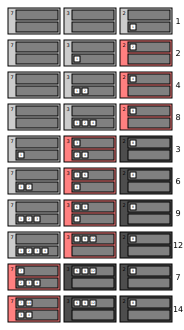
\includegraphics[width=12cm]{linear.pdf}
    \caption[Průběh algoritmu pro generaci nesoudělných čísel]{Průběh algoritmu pro generaci nesoudělných čísel pro $P=\left<2;3;7\right>$ a $m=15$. Každý řádek představuje jeden krok algoritmu. V každém řádku jsou znázorněny všechny továrny zprava doleva. Každá továrna obsahuje svoje prvočíslo $p_a$ a fronty $Q_a$ (dole) a $Z_a$ (nahoře). V každém kroku je aktivována jedna továrna, která je znázorněna červeně. Číslo, které továrna při aktivaci vypíše, je zobrazeno vpravo.}
    \label{figure:linear-steps}
\end{figure}

Tento algoritmus poběží v lineárním čase ku počtu vypsaných čísel. To můžeme dokázat sledováním \enquote{života} čísla v průběhu algoritmu. Číslo začíná svůj život hned potom, co je vypsáno, a je vloženo buď do některé zpětnovazebné fronty $Z_a$ nebo do počáteční fronty $Q_1$. Poté pokaždé, co je z nějaké fronty odebráno, tak buď vypíšeme nové číslo a vrátíme ho do jiné fronty, anebo ho navždy zahodíme. Manipulací s frontou tedy provede algoritmus řádově lineárně.

\subsection{Časová složitost}

Algoritmus má dva hlavní kroky, a to Eratosthenovo síto a generace zlomků.

Smyčka procházející jednotlivé jmenovatele nás nic navíc nestojí, jelikož při každém průchodu vypíšeme minimálně zlomek ve tvaru $\frac{1}{m}$. Už jsem zmiňoval, že čas potřebný k generaci povolených prvočísel je zanedbatelný.

Získáme tedy časovou složitost $O\left(k + n \log{n}\right)$.

Uvažujme všechny zlomky ve tvaru $\frac{2^a}{2b+1}; 2^a \in \left(0; \frac{n}{2}\right); 2b+1 \in \left(\frac{n}{2}; 1\right)$. Všechny tyto zlomky jsou zjevně v základním tvaru a menší než jedna. Snadno také můžeme určit, že je jich řádově $O\left(n \log{n}\right)$. Jelikož je množina těchto zlomů podmnožinou vypsaných zlomků, tak platí, že $O\left(k\right) \geq O\left(n \log{n}\right)$.

$O\left(n \log{n}\right)$ tedy můžeme z časové složitosti vynechat a získáme $O\left(k\right)$. Tato časová složitost je zjevně optimální.

\subsection{Paměťová složitost}
\label{section:memory}

Jakmile dogenerujeme nesoudělná čísla pro jednoho jmenovatele, tak můžeme všechny fronty zapomenout. Jelikož platných zlomků s jmenovatelem $m$ existuje nejvýše $m$ a $m < n$, tak jedno volání algoritmu pro generaci nesoudělných čísel trvá nejdéle $O\left(n\right)$, z čehož vyplývá, že potřebuje nejvýše $O\left(n\right)$ paměti.

Tuto složitost nám však kazí tabulka získaná Eratosthenovým sítem, která zabírá $O\left(n \log{n}\right)$ paměti. Naštěstí můžeme Eratosthenovo síto nahradit algoritmem se stejnou časovou složitostí, který bude prvočíselný rozklad generovat online.

Podobně jako u Eratosthenova síta si vytvoříme seznam hašovacích tabulek $H$ s prvky $H_2$ až $H_n$.

Budeme tento seznam postupně procházet. Pro každé $m$ od $2$ do $n$ provedeme následující kroky:

\begin{enumerate}
    \item Pokud je $H_m$ prázdné, přidáme do něj $m$
    \item Vypíšeme $H_m$
    \item Pro každý prvek $p$ v $H_m$:
          \begin{enumerate}[label*=\arabic*.]
              \item Přídáme $p$ do $H_{m+p}$
          \end{enumerate}
    \item Vyprázdníme $H_m$
\end{enumerate}

Tento algoritmus funguje podobně jako Eratosthenovo síto, akorát je každé prvočíslo v libovolný okamžik uloženo jen u jednoho jeho násobku, a to vždy toho následujícího. Časová složitost tohoto algoritmu je stále $O\left(n \log{n}\right)$, zatímco paměťová je jen $O\left(n\right)$.

Tím jsme snížili paměťovou složitost celého algoritmu na $O\left(n\right)$.

\subsection{Implementace}

Zde je implementace v jazyce Python:

\inputminted{python}{code/linear.py}

\section{Generace začátku posloupnosti (35-1-X1)}

Nyní máme za úkol vygenerovat jen prvních $k$ prvků, navíc seřazených vzestupně. Náš algoritmus upravíme tak, aby prvky generoval onlinově v seřazeném pořadí. Jakmile vypíšeme $k$ prvků, tak program ukončíme.

Použijeme verzi algoritmu bez optimalizace uvedené v \ref{section:memory}, tj. s Eratosthenovým sítem.

\subsection{Generace nesoudělných čísel, seřazených vzestupně}

Nyní se nám bude hodit \enquote{továrnový} model našeho algoritmu znázorněný v obrázku \ref{figure:linear-steps}. Každá továrna sama o sobě vypisuje čísla seřazená. Stačí nám tedy továrny aktivovat ve správném pořadí.

Opět vypočítáme seznam platných prvočísel, jak je uvedeno v sekci \ref{section:valid-primes}. Dále vytvoříme seznam $r$ továren.\footnote{Připomínám, že $r$ je počet prvočísel.} Každé prvočíslo bude mít svoji továrnu. Továrna $T_a$ bude obsahovat svoje prvočíslo $p_a$ a fronty $Q_a$ a $Z_a$. Na začátek vypíšeme jedničku a vložíme ji do fronty $Q_1$. Pro každou továrnu jsme schopni v konstantním čase určit, jaké číslo vypíše jako další (jestli vůbec). Jak vypadá tento seznam můžete vidět na obrázku \ref{figure:factories}.

\begin{figure}[hp]
    \centering
    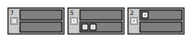
\includegraphics[width=15cm]{array.pdf}
    \caption[Seznam továren]{Seznam továren. Každá továrna má svoje prvočíslo $p_a$ vlevo nahoře a fronty $Q_a$ a $Z_a$. V čtverečkovaném rámečku je uvedeno číslo, které továrna vygeneruje při další aktivaci.}
    \label{figure:factories}
\end{figure}

Vytvoříme si haldu, ve které budeme ukládat odkazy na továrny. Budeme je řadit podle předpovídaného dalšího čísla. Továrny, které mají obě fronty prázdné, umístíme dospod, jako by bylo jejich další číslo nekonečno.\footnote{Alternativně nemusí být takové továrny v haldě vůbec, ale bylo by zbytečně hodně práce je ve správnou chvíli do haldy vracet.} Předpovídané další číslo továrny se může změnit, pokud přidáme nové číslo do některé z jejích front. V tom případě nesmíme zapomenout pozici továrny v haldě poopravit, což zvládneme v $O\left(\log{r}\right)$.\footnote{Zatímco snižování klíče v haldě je častá a známá operace, zvyšování klíče se používá málokdy. Možné to nicméně je.} Musíme však být schopni v rozumném čase danou továrnu v haldě najít, a tak si budeme stranou pro každou továrnu pamatovat její pozici v haldě.\footnote{Pokud máme haldu implementovanou v podobě seznamu, tak se pozice prvků v paměti neustále mění. Pokud však máme haldu uloženou jako klasický strom, tak může každá továrna dostat stabilní lokaci v paměti.}\footnote{Další možností je použít jinou implementaci prioritní fronty, například vyvážený binární vyhledávací strom.}

Budeme vždy aktivovat továrnu na vrcholu haldy, dejme tomu $T_a$, a necháme ji vypsat další číslo. Potom poopravíme pozici $T_a$ a $T_{a+1}$ v haldě. Skončíme, jakmile příští číslo továrny na vrcholu haldy přesáhne $m$. Ukázkový průběh tohoto algoritmu najdete na obrázku \ref{figure:selected-steps}.

\begin{figure}[hp]
    \centering
    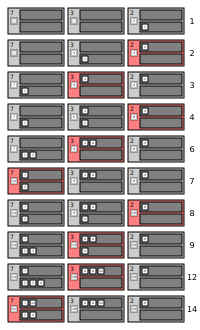
\includegraphics[width=12cm]{selected.pdf}
    \caption[Průběh algoritmu pro generaci seřazených nesoudělných čísel]{Průběh algoritmu pro generaci seřazených nesoudělných čísel. Každý řádek představuje jeden krok algoritmu. Řadek zobrazuje stav po aktivaci jedné z továren. Aktivovaná továrna je označená červeně, vypsané číslo je uvedeno vpravo.}
    \label{figure:selected-steps}
\end{figure}

Dosáhli jsme toho, že budou všechna čísla vypsána ve správném pořadí. Může nás napadnout, jestli se nemůže stát, aby nějaké továrně do její vstupní fronty nějaké číslo nedorazilo \enquote{včas}. Nicméně libovolné číslo $x$ předá továrna $T_{a-1}$ továrně $T_a$ v okamžiku, kdy vypíše číslo $x p_{a-1}$. Továrna $T_a$ toto číslo potřebuje až v okamžiku, kdy má za úkol vypsat číslo $x p_a$. Jelikož $p_{a-1} < p_{a}$, a tedy $x p_{a-1} < x p_{a}$, tak továrna $T_a$ dostane $x$ vždy před tím, než ho potřebuje.

\subsection{Generace zlomků, seřazených vzestupně}

Máme tedy algoritmus, který postupně generuje platné jmenovatele zlomků s daným čitatelem. Tento algoritmus spustíme paralelně $n-1$ krát, jednou pro každého jmenovatele od $2$ do $n$. Zlomky $\frac{0}{1}$ a $\frac{1}{1}$ vypíšeme zvlášť na začátku a na konci. Generátory čitatelů pojmenujeme $G_2$ až $G_n$.

Pro každý generátor jsme schopni snadno určit další číslo, které vygeneruje. To uděláme buď tak, že se podíváme na klíč vrcholu haldy továren, a nebo prostě tak, že necháme každý generátor vždy vygenerovat jedno číslo dopředu.

Podobně jako u továren vytvoříme z generátorů haldu. Budeme ji řadit podle dalšího zlomku, který vygenerují, tj. jejich další číslo děleno jejich jmenovatelem. Z vrcholu této haldy vždy vybereme generátor, vypíšeme jeho další zlomek, posuneme jeho stav o jeden krok a vrátíme ho na správné místo v haldě (pokud nedoběhl). To budeme opakovat, dokud nevypíšeme $k$ zlomků. Pokud doběhnou všechny generátory, tak vypíšeme $\frac{1}{1}$. Pokud jsme v tu chvíli stále ještě nevypsali $k$ zlomků, tak jsme dostali na vstupu neplatné $k$.

\subsection{Časová složitost}

Zde je přehled časových složitostí jednotlivých operací:

\begin{itemize}
    \item Eratosthenovo síto - $O\left(n\log{n}\right)$
    \item Vytvoření generátorů - $O\left(n\right)$ krát:
          \begin{itemize}
              \item Nalezení platných prvočísel - $O\left(r\right)$
              \item Vytvoření seznamu továren - nejhůře $O\left(r\right)$
              \item Vytvoření haldy továren - nejhůře $O\left(r\right)$\footnote{Haldu postavíme v $O\left(n\right)$, neboť všechny prvky až na jeden budou nekonečno.}
          \end{itemize}
    \item Generování zlomků - $O\left(k\right)$ krát:
          \begin{itemize}
              \item Určení dalšího generátoru - $O\left(\log{n}\right)$
              \item Určení další továrny - $O\left(\log{n}\right)$
              \item Vypočítání nového čitatele - $O\left(1\right)$
              \item Úprava pozice továren v haldě - $O\left(\log{n}\right)$
              \item Vrácení generátoru do haldy - $O\left(\log{n}\right)$
          \end{itemize}
\end{itemize}

Eratosthenovo síto a generování zlomků má tedy složitost $O\left(k\log{n} + n\log{n}\right)$. Zadání garantuje, že $k \geq n$, takže složitost můžeme zjednodušit na $O\left(k\log{n}\right)$.

Doba potřebná k vytvoření generátorů je lineární ku celkovému počtu platných prvočísel.\footnote{Plus $O\left(n\log{n}\right)$, ale to se stejně jako v sekci \ref{section:valid-primes} ztratí v době běhu Eratosthenova síta.} Když jsme generovali celou posloupnost, tak jsme se mohli spolehnout na to, že jich bude méně než vypsaných zlomků. Teď už to však nutně neplatí. Platná prvočísla tedy budeme generovat, až když budou potřeba. Při inicializaci generátoru najdeme jen nejmenší platné prvočíslo, což zvládneme v konstantním čase.\footnote{Doba potřebná k přeskočení neplatných prvočísel se zase schová v době běhu Eratosthenova síta.} Na začátku tedy budeme mít v haldě jen jednu továrnu. Jakmile se pokusí poslední továrna předat číslo neexistující další továrně, tak najdeme další platné prvočíslo a vytvoříme továrnu novou. Pochopitelně přestaneme, jakmile dojdou platná prvočísla, a budeme dále předávaná čísla zahazovat.

Tím se nám podařilo dobu běhu zredukovat na $O\left(k\log{n}\right)$.

\subsection{Paměťová složitost}

V paměti máme uložené následující informace:

\begin{itemize}
    \item Prvočíselné rozklady - $O\left(n\log{n}\right)$
    \item Haldu generátorů - $O\left(n\right)$
    \item Haldy továren - $O\left(k\right)$
    \item Čísla ve frontách - $O\left(k\right)$
\end{itemize}

Paměťová složitost je tedy $O\left(k + n\log{n}\right)$.

Tento odhad můžeme mírně zlepšit přesnějším odhadem časové a tedy i paměťové složitosti Eratosthenova síta. Zatím jsme pracovali se snadno dokazatelnou horní mezí složitosti $O\left(n\log{n}\right)$, nicméně bylo dokázáno,\footnote{Viz \url{https://en.wikipedia.org/w/index.php?title=Sieve_of_Eratosthenes&oldid=1107644292\#Algorithmic_complexity}.} že je jeho složitost jen $O\left(n\log{\log{n}}\right)$. S využitím tohoto důkazu můžeme odhad paměťové složitosti zredukovat na $O\left(k + n\log{\log{n}}\right)$.

\section{Porovnání s optimálním algoritmem}

Na Wikipedii můžeme najít algoritmus\footnote{Viz \url{https://en.wikipedia.org/w/index.php?title=Farey_sequence&oldid=1110352333\#Next_term}.}, který využívá matematických vztahů mezi sousedními zlomky k tomu, aby vygeneroval prvních $k$ prvků Fareyovy posloupnosti s časovou složitostí $O\left(k\right)$ a paměťovou složitostí $O\left(1\right)$. Tento algoritmus je zjevně optimálním řešením pro obě úlohy.

Můj algoritmus pro generování celé posloupnosti má stejnou časovou složitost jako tento algoritmus, zato můj algoritmus pro generování začátku je $O\left(\log{n}\right)$ krát pomalejší. Oba moje algoritmy mají výrazně horší paměťovou složitost, a to zvlášť ten druhý.

\end{document}
